\subsection{Current adapter admission decisions}\label{app:live-adapter-decisions}

Complete entries in the summary, adapter-admission and \mbox{per-round}
journals supply the scalar decisions in \cref{fig:fw-live-adapter-decisions}.

\begin{figure}[!tb]
  \centering
  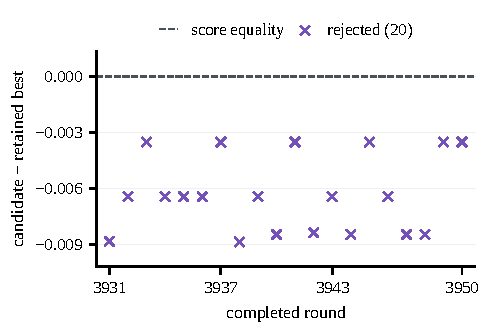
\includegraphics[width=\linewidth]{figures/fig_fw_live_adapter_decisions.pdf}
  \caption{\textbf{All 20 candidates in the window are rejected.}
  Rounds 3931--3950, captured at 23:00 UTC on 2 November 2026.
  Each point is candidate validation-pool utility minus the pre-decision retained best;
  zero denotes equality. Markers show logged admission decisions, with
  all 20 candidates rejected. Retained-best utility remains \num{1.1389572}.
  This adaptive window does not measure \mbox{independent}
  first-proposal or serving performance. Scope: \cref{sec:method-status}.}
  \label{fig:fw-live-adapter-decisions}
\end{figure}

The full admission record follows retained utility from round 775
(\cref{fig:fw-retained-best-plateau}).
\Cref{fig:fw-pool-insertions} separately counts pool insertions and adapter
rejections in its stated historical window.

\begin{figure}[!tb]
  \centering
  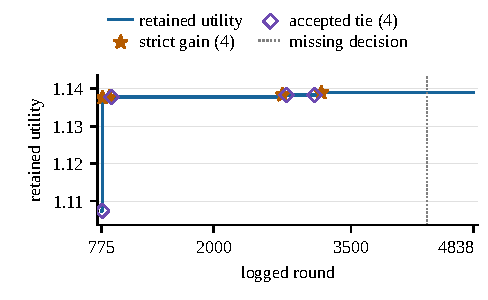
\includegraphics[width=\linewidth]{figures/fig_fw_retained_best_plateau.pdf}
  \caption{\textbf{Four strict gains and four ties mark the retained-utility record.}
  All \num{4063} logged adapter decisions in rounds 775--4838, captured
  at 04:56 UTC on 4 November 2026. Blue: post-decision retained utility;
  stars: strict gains; diamonds: accepted ties. Round 4331 is absent;
  the curve does not bridge it. Every recorded score is used, without a
  cumulative maximum or smoothing. This adaptive development record is not
  independent first-proposal or learning-gain evidence. Scope: \cref{sec:method-status}.}
  \label{fig:fw-retained-best-plateau}
\end{figure}

\begin{figure}[!tb]
  \centering
  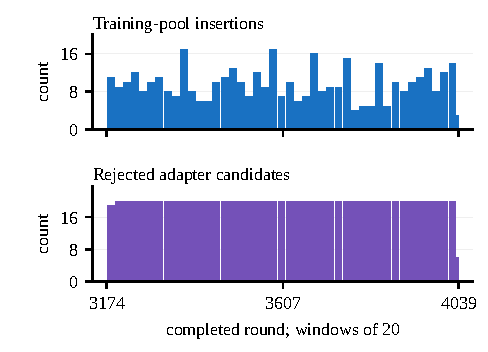
\includegraphics[width=\linewidth]{figures/fig_fw_pool_insertions.pdf}
  \caption{\textbf{Pool insertions and adapter rejections count different events.}
  Rounds 3174--4039, from complete journal prefixes captured on
  3 November 2026. Top: 421 logged automatic training-pool insertion
  events. Bottom: 865 rejected adapter candidates out of 866 decisions.
  Bars sum 20 consecutive completed rounds; the final bar covers six.
  Program-level insertions (events per window) and adapter rejections
  (decisions per window) have different units.
  These adaptive counts do not measure independent first-proposal
  \mbox{or learning gains. Scope: \cref{sec:method-status}.}}
  \label{fig:fw-pool-insertions}
\end{figure}
